\documentclass[aps,prb,groupedaddress,twocolumn,showpacs,dvipdfmx,superscriptaddress,pdftex]{revtex4-2}
\usepackage[whole]{bxcjkjatype}
\usepackage{amsmath}
\newcommand\numberthis{\addtocounter{equation}{1}\tag{\theequation}}
\usepackage{amssymb}
\usepackage{bm}
\usepackage{dcolumn}
\usepackage{graphicx}
\usepackage{bm}
\usepackage{url}
\usepackage{here}
\usepackage{multirow}
\usepackage{ulem}
\usepackage{booktabs}
\usepackage[T1]{fontenc}
\usepackage[caption=false]{subfig}
\usepackage[usenames,dvipsnames]{color}
\usepackage{tabularray}
\usepackage{fvextra}
% \usepackage{pdfpages}
% \usepackage{epstopdf}
% \epstopdfDeclareGraphicsRule{.pdf}{png}{.png}{convert #1 \OutputFile}
% \AppendGraphicsExtensions{.pdf}
% \usepackage{hyperref}

% tiếng Việt
\usepackage[T5]{fontenc}
\usepackage[utf8]{inputenc}
\DeclareTextSymbolDefault{\DH}{T1}
%-------------------------------------
\newcommand{\tadd}[1]{\textcolor{red}{#1}}
\newcommand{\trem}[1]{{\color{red}\sout{#1}}}
\newcommand{\tcom}[1]{\textcolor{red}{\textbf{TI: #1}}}
\newcommand{\citehere}{\textcolor{red}{\textbf{(citation)}}}
\newcommand{\x}{\times}
%-------------------------------------
% \newcommand{\ghost}[1]{[#1]}
\newcommand{\ghost}[1]{}
%----------------------------------------
\def\red{\color{red}}
\def\blue{\color{blue}}
\def\green{\color{green}}
%%%%%%%%%%%%%%%%%%%%%%%%%%%%%%%%%%%%%%%%%
\begin{document}
\title{
    Meta-learning in movement prediction problem of aperiodic time-series data
}
%%%%%%%%%%%%%%%%%%%%%%%%%%%%%%%%%%%%%%%%%
\author{Bao-Long Nguyen}
\email{mwklng2309@icloud.com}
\affiliation{School of Information Science, JAIST, Ishikawa, Japan}
%
\author{Tom Ichibha}
\email{ichibha@icloud.com}
\affiliation{School of Information Science, JAIST, Ishikawa, Japan}
%
\author{Kenta Hongo}
\email{kenta_hongo@mac.com}
\affiliation{Research Center for Advanced Computing Infrastructure, JAIST, Ishikawa, Japan}
%
\author{Ryo Maezono}
\email{rmaezono@mac.com}
\affiliation{School of Information Science, JAIST, Ishikawa, Japan}
%
\date{\today}
%%%%%%%%%%%%%%%%%%%%%%%%%%%%%%%%%%%%%%%%%
\begin{abstract}

    \textbf{Abstract}. Dự đoán aperiodic time-series data (e.g. stock price, foreign exchange, Bitcoin price,...) là một tác vụ khó khăn đối với các mô hình học máy bởi vì loại dữ liệu này có phương sai cao và không cố định; không thể hiện chu kỳ rõ ràng nên khó rút trích đặc trưng; không chỉ phụ thuộc vào giá trị quá khứ mà còn phụ thuộc các yếu tố khác, điều khiến chúng bất ổn và không có chu kỳ như tình hình kinh tế, chính trị. Để khắc phục các thách thức nêu trên, chúng tôi sử dụng Meta-learning để huấn luyện kết hợp mạng \verb|LSTM| và \verb|CNN|, từ đó rút trích và tổng hợp hiệu quả các đặc trưng ẩn của dữ liệu theo thời gian. Thực nghiệm trên dữ liệu foreign exchange của 15 cặp tiền tệ trong vòng 24 năm (2000-2024) cho thấy phương pháp đề xuất hoạt động tốt và có độ chính xác cao hơn mô hình \verb|NHITS| - state-of-the-art (SOTA) model của năm 2023 trên dữ liệu time-series, trong bài toán dự đoán xu hướng (upward or downward) của ngày giao dịch tiếp theo.

\end{abstract}
%----------------------------------------
\keywords{Meta-learning, \verb|LSTM|, \verb|CNN|, Aperiodic time-series data, Foreign exchange}
\maketitle

%%%%%%%%%%%%%%%%%%%%%%%%%%%%%%%%%%%%%%%%%
\section{Introduction}
\label{sec.intro}
%%%%%%%%%%%%%%%%%%%%%%%%%%%%%%%%%%%%%%%%%

Aperiodic time-series prediction nói chung hay foreign exchange (FX) prediction nói riêng từ lâu đã là vấn đề đáng quan tâm của nhiều nghiên cứu \citep{li2019multi, islam2021foreign, heryadi2021foreign}. Hai kỹ thuật chính được sử dụng trong aperiodic time-series prediction là fundamental analysis and technical analysis \cite{ayitey2023forex}. Trong khi fundamental analysis thiên về phân tích các yếu tố tác động từ bên ngoài và khó có thể capture từ các biến thiên giá trị trong quá khứ như chính sách, chiến lược kinh tế của công ty, quốc gia để dự đoán tương lai; technical analysis dựa hoàn toàn vào lịch sử biến động giá trị để phân tích xu hướng tương lai.

\vspace{2mm}

Việc dự đoán trên aperiodic time-series data gặp một vài thách thức cố hữu. Trong đó có thể kể tới: (1) - Variance của loại dữ liệu này biến thiên mạnh qua các thời kỳ. Từ đó giả thuyết rằng chúng tuân theo một phân phối để có thể xấp xỉ lỗi là không thể sử dụng được, dẫn đến việc các mô hình học máy khó có thể dự đoán chính xác giá trị cũng như xu hướng trong tương lai; (2) - Aperiodic data không tuân theo bất kỳ quy luật rõ ràng nào nên việc học các đặc trưng ẩn của dữ liệu để tiến hành dự đoán gặp rất nhiều khó khăn; (3) - Aperiodic time-series data (e.g. giá cổ phiếu của một công ty) không hoàn toàn phụ thuộc vào dữ liệu quá khứ mà còn phụ thuộc nhiều yếu tố ngoại lai (e.g. tin tức, tình hình kinh tế, chính trị) \cite{li2019multi}.

\vspace{2mm}

Đối với thách thức đầu tiên, các mô hình ensemble [cite something here] thường được sử dụng để hạn chế ảnh hưởng của sự biến đổi variance. Ensemble model giúp cung cấp một cái nhìn tổng quát, tổng hợp từ nhiều khía cạnh dựa trên các sub-models, từ đó giúp mô hình tổng quát thích ứng được với sự thay đổi mạnh của variance. Chúng tôi tiếp cận bài toán theo hướng này nhưng ở mức cao hơn bằng cách sử dụng Meta-learning (ML) \cite{finn2017model}. Phương pháp này tổng hợp hiệu quả tham số của các mô hình cục bộ, giúp giảm thiểu đáng kể variance loss.

\vspace{2mm}

Để khắc phục thách thức thứ hai, các nghiên cứu phần lớn sử dụng các đặc trưng rút trích được từ Long short-term memory neural network (\verb|LSTM|) \cite{hochreiter1997long}, Artificial neural network (\verb|ANN|), và Convolution neural network (\verb|CNN|) \cite{lecun1989handwritten}. Cụ thể, trong năm 2022, 20\% tổng số các bài báo liên quan đến dự đoán chỉ số tài chính sử dụng \verb|LSTM|, 20\% sử dụng \verb|ANN| và 6\% sử dụng \verb|CNN| \cite{ayitey2023forex}. Để tận dụng hết được các đặc trưng được rút trích bởi các mô hình nêu trên, chúng tôi đề xuất phương pháp kết hợp các đặc trưng này.

\vspace{2mm}

Đối với thách thức thứ ba, nghiên cứu \cite{fama1970efficient} đưa ra giả thuyết rằng các time-series datasets khác nhau của cùng một lĩnh vực tại cùng thời điểm phản ánh sự tác động của các yếu tố ngoại lai. Ví dụ, các nghiên cứu \citep{overreactioncontrarian, mech1993portfolio} cũng chỉ ra sự phụ thuộc giữa chỉ số tài chính của một công ty nhất định và các chỉ số của các công ty khác. Điều này càng làm tăng tính đúng đắn của giả thuyết trong nghiên cứu \cite{fama1970efficient}. Ngoài ra, chúng tôi cho rằng, loại dữ liệu này còn có những phụ thuộc ngầm vào các thời điểm nhất định trong quá khứ (hidden long-term dependency). Đối với cách tiếp cận truyền thống, người ta sử dụng một lượng dữ liệu quá khứ cố định (lookback window) để huấn luyện mô hình. Điều này gây một trở ngại lớn cho quá trình học vì các đặc trưng dài hạn theo thời gian sẽ bị quên. Mặt khác, ML chia nhỏ tập dữ liệu thành nhiều phần để học và tổng hợp hiệu quả các tham số học được nên có thể xử lý tốt thách thức này.

\vspace{2mm}

Cuối cùng, chúng tôi chứng minh tính ưu việt của thuật toán đề xuất bằng cách giải bài toán dự đoán xu hướng (tăng hoặc giảm) của tỉ giá ngoại hối và so sánh kết quả với mô hình SOTA hiện tại (\verb|NHITS| \cite{challu2023nhits}) trên hai loại dữ liệu: (1) - Dữ liệu tỉ giả của cặp tiền tệ USD/JPY; (2) - Dữ liệu tỷ giá của 60 cặp tiền tệ, cấu thành từ 18 quốc gia. Các tập dữ liệu này được công khai trên Internet và có thể tải về dễ dàng. Bản cài đặt chính thức có thể xem tại [bỏ cái link github vào đây].

\vspace{2mm}

Tóm lại, đóng góp chính của chúng tôi như sau:

\begin{itemize}
    \item Kết hợp đặc trưng: Rút trích đặc trưng bằng cách kết hợp các đặc trưng của \verb|LSTM| và \verb|CNN|.
    \item Hidden long-term dependency: Chứng minh thực nghiệm rằng một aperiodic time-series data nhất định không chỉ phụ thuộc vào các yếu tố ngoại lai mà còn có các phụ thuộc ẩn với chính nó tại nhiều thời điểm khác nhau trong quá khứ.
    \item Tổng hợp hiệu quả tham số mô hình: Sử dụng ML thay cho các mô hình ensemble truyền thống trong việc tổng hợp kết quả từ các mô hình học máy.
    \item Experiment: Thực nghiệm trên các bộ dữ liệu về tỉ giá hối đoái và so sánh với mô hình SOTA \verb|NHITS| để chứng minh tính hiệu quả của phương pháp đề xuất.
\end{itemize}

%%%%%%%%%%%%%%%%%%%%%%%%%%%%%%%%%%%%%%%%%%%%%%%%%%%%
\section{Related work}
\label{sec.relatedWork}
%%%%%%%%%%%%%%%%%%%%%%%%%%%%%%%%%%%%%%%%%%%%%%%%%%%%

\subsection{LSTM \& CNN model}

Như đã đề cập, \verb|LSTM| là mạng neural rất phổ biến trong việc handle các bài toán liên quan đến dự đoán trên dữ liệu time-series. \verb|LSTM| được sử dụng phổ biến như vậy bởi vì nó xử lý tốt vấn đề vanishing gradient (dễ dàng bắt gặp khi sử dụng Recurrent neural network) và có thể khai thác hiệu quả các mối quan hệ phi tuyến trong dữ liệu. Thật vậy, bằng cách duy trì cell-state trong mỗi iteration, \verb|LSTM| có thể khắc phục vấn đề vanishing gradient, từ đó bảo toàn khả năng capture các phụ thuộc dài hạn \cite{cheng2018applied}. Ngoài ra, \verb|LSTM| thực hiện rút trích đặc trưng với các hàm kích hoạt phi tuyến, giúp các tham số mô hình có thể capture tính phi tuyến của dữ liệu \cite{he2016exploiting}. Hai yếu tố nêu trên khiến cho \verb|LSTM| trở thành lựa chọn đầu tiên được nghĩ đến khi giải quyết các bài toán trên dữ liệu time-series.

\vspace{2mm}

Mạng \verb|CNN| được sử dụng rất nhiều trong các tác vụ xử lý hình ảnh \citep{naranjo2020review, sharma2018analysis} bởi khả năng tổng hợp các quan hệ cục bộ. Không chỉ vậy, \verb|CNN| còn được dùng rất nhiều trong các tác vụ xử lý dữ liệu time-series như speech recognition \cite{dua2022developing}, natural language processing \cite{varshitha2023natural}. Điều đó chứng tỏ được khả năng của \verb|CNN| trong việc khám phá mối quan hệ thời gian cục bộ giữa các mẫu dữ liệu. Mặc dù vậy, \verb|CNN| lại rất ít được dùng trong các tác vụ dự đoán stock price hay foreign exchange. Trong nghiên cứu này, chúng tôi tận dụng khả năng rút trích đặc trưng cục bộ tuyệt vời của \verb|CNN| để tích hợp thêm thông tin ẩn vào quá trình huấn luyện của mô hình.

\subsection{Model-agnostic Meta-learning (MAML)}

Các thuật toán Meta-learning (ML), điển hình là MAML \cite{finn2017model} được biết đến với khả năng huấn luyện một mô hình có tính tổng quát cao, thích ứng nhanh trên tập dữ liệu mới thông qua một lượng nhỏ dữ liệu và số bước huấn luyện \citep{hospedales2021meta, vettoruzzo2024advances}. Với khả năng này, ML được sử dụng rất nhiều trong các tác vụ đòi hỏi khả năng đáp ứng của mô hình trên dữ liệu (e.g. cá nhân hóa mô hình học \citep{chen2018federated, fallah2020personalized,nguyen2022meta}, domain adaptation trong online learning \citep{hu2023meta, khoee2024domain}).

\vspace{2mm}

Một thuật toán ML cơ bản sẽ được học trên nhiều tác vụ $t$ rút ra từ cùng một phân phối tác vụ $\mathcal{T}$ \cite{hospedales2021meta}. Dữ liệu của mỗi tác vụ được chia thành tập support $\mathcal{D}_t^{support}$ (thường có kích thước nhỏ, khoảng 20\%) và tập query $\mathcal{D}_t^{query}$. Trong qua trình học, hai bước tối ưu inner và outer optimization được perform đan xen. Inner optimization cố gắng tìm ra một bộ tham số tối ưu $\theta_t^*$ cho từng mô hình học máy trên tập support của mỗi tác vụ bằng phương trình \ref{eq:inner_opt}.

\begin{equation}
    \theta_t^* = \theta_t(\phi) = \arg\min_{\theta}{\mathcal{L}^{task}_t\left( \phi, \mathcal{D}_t^{support} \right)}
    \label{eq:inner_opt}
\end{equation} Trong đó, $\phi$ là kết quả của quá trình outer optimization, đóng vai trò là giá trị khởi tạo của $\theta_t$. $\mathcal{L}_t$ là hàm lỗi của mô hình trên tác vụ $t$.

\vspace{2mm}

Sau đó, thuật toán sử dụng các bộ tham số tối ưu $\theta_t^*$ để perform trên tập query tương ứng. Lỗi của toàn bộ mô hình sau đó được tổng hợp để thực hiện quá trình outer optimization như phương trình \ref{eq:outer_opt}.

\begin{align*}
    \phi^* &= \arg\min_{\phi}\sum_{t}{\mathcal{L}^{meta}_t\left[ \theta_t^*, \mathcal{D}_t^{query} \right]}\\
    &= \arg\min_{\phi}\sum_{t}{\mathcal{L}^{meta}_t\left[ \theta_t(\phi), \mathcal{D}_t^{query} \right]} \numberthis
    \label{eq:outer_opt}
\end{align*}

Trong inference phase, giá trị khởi tạo cho tham số của mô hình được gán bằng $\phi^*$. Mô hình sau đó được huấn luyện nhanh trên tập support sau đó perform trên tập query. Kết quả trên tập query chính là kết quả của mô hình.

\vspace{2mm}

Bằng hình thức huấn luyện trên, mô hình $\phi^*$ sẽ có mức tổng quát hóa cao trên các tác vụ khác nhau, có thể nhanh chóng đáp ứng một tác vụ mới chỉ sau một vài bước huấn luyện.

\vspace{2mm}

Các mô hình hybrid ensemble vốn được sử dụng rất nhiều trong các bài toán xử lý time-series và được chứng minh thực nghiệm là có độ chính xác cao hơn so với các mô hình handle time-series data tiêu chuẩn vì có thể tổng hợp được sức mạnh của nhiều mô hình \cite{ayitey2023forex}. Tuy vậy, các hình thức tổng hợp của ensemble model hiện nay vẫn còn rất cứng nhắc vì chỉ có thể tổng hợp dựa trên kết quả cuối (cơ chế voting của bagging models) và kết quả gần cuối (đối với stacking models). Dưới góc nhìn của ensemble model, có thể coi phương trình \ref{eq:outer_opt} là một phương pháp tổng hợp hiệu quả các sub-model, giúp tận dụng khả năng rút trích đặc trưng của từng mô hình. Nói cách khác, mô hình sau khi tổng hợp có thể rút trích đặc trưng ở mức sâu hơn, cải thiện đáng kể khả năng dự đoán so với các mô hình ensemble truyền thống.

\subsection{Neural Hierarchical Interpolation\\for Time Series (NHITS)}

NHITS được thiết kế để hướng đến việc dự đoán các long-horizon time-series data. Theo nghiên cứu \cite{challu2023nhits}, cấu trúc của \verb|NHITS| bao gồm nhiều stack liên tiếp nhau. Mỗi stack bao gồm nhiều block nối tiếp nhau. Tại mỗi block, dữ liệu lịch sử được sử dụng để dự đoán dữ liệu tương lai và dữ liệu quá khứ. Cụ thể, tại block $l$, với $L$ mẫu dữ liệu quá khứ ($\mathbf{y}_{t-L:t, l-1}$), các đặc trưng sẽ được rút trích như sau (theo \cite{challu2023nhits}):

\begin{align}
    \mathbf{y}_{t-L:t, l}^{(p)} &= \mathbf{Pooling}\left( \mathbf{y}_{t-L:t, l-1} \right)\\
    % \mathbf{h}_l &= FullyConnected\left( \mathbf{y}_{t-L:t, l}^{(p)} \right)\\
    \mathbf{\theta}_l^b &= \mathbf{FullyConnected}^b \left( \mathbf{y}_{t-L:t, l}^{(p)} \right)\\
    \mathbf{\theta}_l^f &= \mathbf{FullyConnected}^f \left( \mathbf{y}_{t-L:t, l}^{(p)} \right)\\
    \mathbf{\hat{y}}_{t-L:t, l} &= g\left(\mathbf{\theta}_l^b\right)\\
    \mathbf{\hat{y}}_{t+1:t+H, l} &= g\left(\mathbf{\theta}_l^f\right)
\end{align}

Trong đó, \verb|FullyConnected| là các lớp multi-layer perception (\verb|MLP|) xếp chồng với hàm kích hoạt phi tuyến. $\mathbf{\theta}_l^f, \mathbf{\theta}_l^b$ là các hệ số nội suy forecast và backcast, được dùng để tổng hợp các giá trị đầu ra của block $l$ bằng hàm nội suy $g(\cdot)$. Đầu ra của block $l$ là giá trị forecast $\mathbf{\hat{y}}_{t+1:t+H, l}$ và giá trị backcast $\mathbf{\hat{y}}_{t-L:t, l}$. Input của block $l+1$ được tính theo phương trình \ref{eq:input_l1}.

\begin{align}
    \mathbf{y}_{t-L:t, l+1} = \mathbf{y}_{t-L:t, l-1} - \mathbf{\hat{y}}_{t-L:t, l}
    \label{eq:input_l1}
\end{align}

Giả sử mô hình gồm có $S$ stacks, mỗi stack có $B$ blocks. Tổng hợp các giá trị forecast của các block như phương trình \ref{eq:sum_block}, ta được giá trị forecast của một stack. Backcast của block cuối cùng của một stack chính là đầu vào cho stack tiếp theo. Cuối cùng, tổng hợp giá trị forecast của các stack như phương trình \ref{eq:sum_stack}, ta được giá trị forecast dự đoán của toàn mạng.

\begin{align}
    \mathbf{\hat{y}}_{t+1:t+H}^s &= \sum_{l=1}^{B}{\mathbf{\hat{y}}_{t+1:t+H, l}} \label{eq:sum_block}\\
    \mathbf{\hat{y}}_{t+1:t+H} &= \sum_{s=1}^{S}{\mathbf{\hat{y}}_{t+1:t+H}^s} \label{eq:sum_stack}
\end{align}

Bằng cách xếp chồng các stack, stack sau nhận vào phần dư của stack trước, kiến trúc trên được kỳ vọng là sẽ phân rã dữ liệu thành các frequency bands khác nhau (weekly, daily, even hourly). Trên thực tế, \verb|NHITS| perform rất tốt đối với các bộ dữ liệu có tính chu kỳ cao như mức tiêu thụ điện, thời tiết, giao thông. Tuy nhiên, chúng tôi đang hướng đến aperiodic time-series dataset, vốn có tính chu kỳ rất thấp, thậm chí không có (see figure \ref{fig:fx}). Điều này gây ra khó khăn rất lớn cho \verb|NHITS|.

\begin{figure}[h]
    \centering
    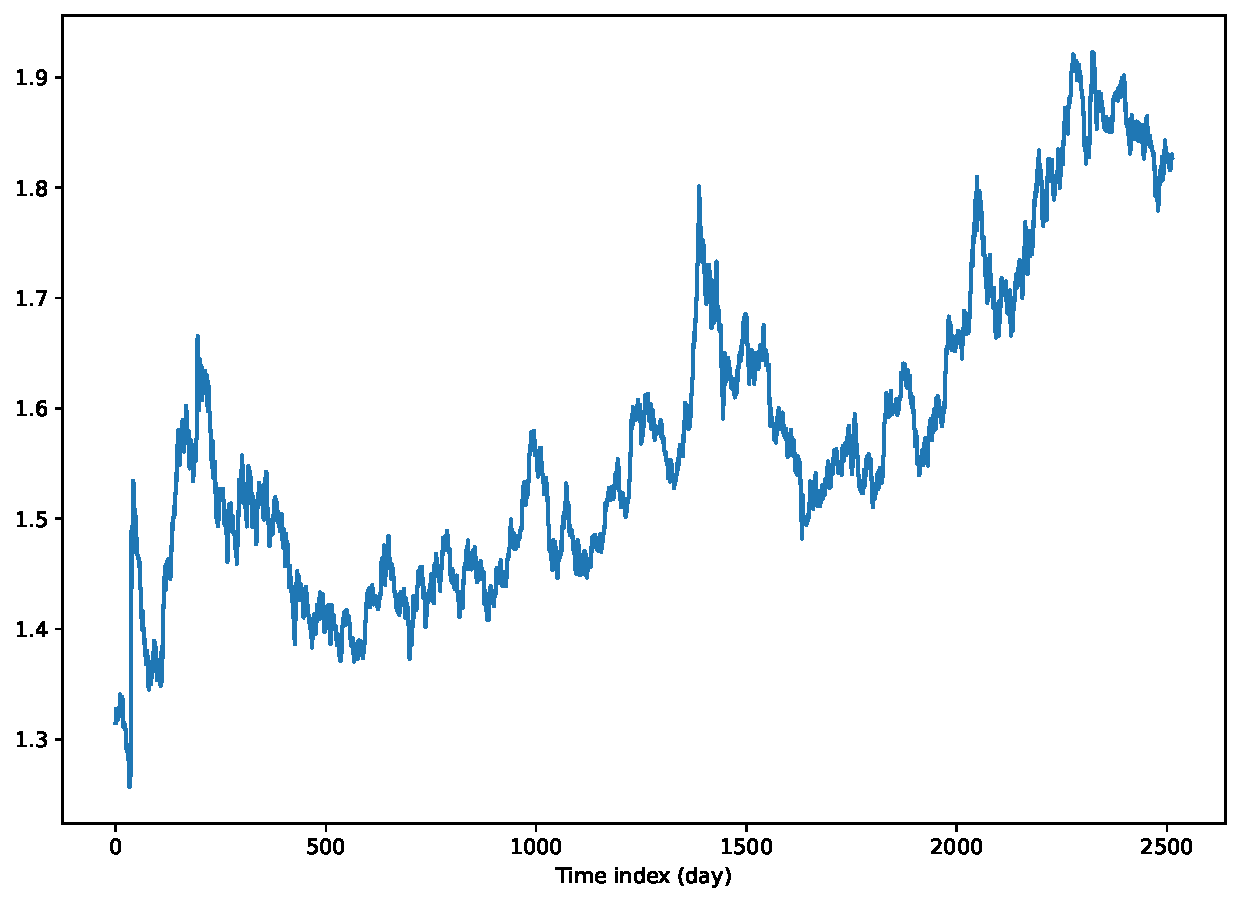
\includegraphics[width=\linewidth]{img/CHF_NZD.pdf}
    \caption{Exchange rate (close price) between Swiss franc and New Zealand dollar by day (2014-2024).}
    \label{fig:fx}
\end{figure}

%%%%%%%%%%%%%%%%%%%%%%%%%%%%%%%%%%%%%%%%%%%%%%%%%%%
\section{Methodology}
\label{sec.method}
%%%%%%%%%%%%%%%%%%%%%%%%%%%%%%%%%%%%%%%%%%%%%%%%%%%

% nói tổng quan ở đây, vẽ cái hình và bỏ vào
Phương pháp của chúng tôi bao gồm hai phần chính hoạt động song song nhau: (1) - Feature extraction; (2) - Parameter synthesis. Tổng quan phương pháp được minh họa trong hình \ref{fig:flow}. Trong phần feature extraction, chúng tôi kết hợp hai loại đặc trưng từ mạng \verb|CNN| và \verb|LSTM|. Trong phần parameter synthesis, chúng tôi sử dụng \verb|MAML| để tổng hợp tham số của các mô hình. Với sự góp mặt của các đặc trưng \verb|LSTM| và \verb|CNN|, chúng tôi kỳ vọng sẽ rút trích được các đặc trưng ẩn trong dữ liệu aperiodic. Bằng việc sử dụng \verb|MAML| trong quá trình tổng hợp trọng số, phương pháp đề xuất được kỳ vọng là một giải pháp thay thế hợp lý và hiệu quả cho các mô hình ensemble truyền thống trong việc giảm thiểu tác động của sự biến thiên variance, tổng hợp hiệu quả các yếu tố ngoại lai, cũng như giữ được các hidden long-term dependency ẩn trong quá khứ.

\begin{figure*}[ht]
    \centering
    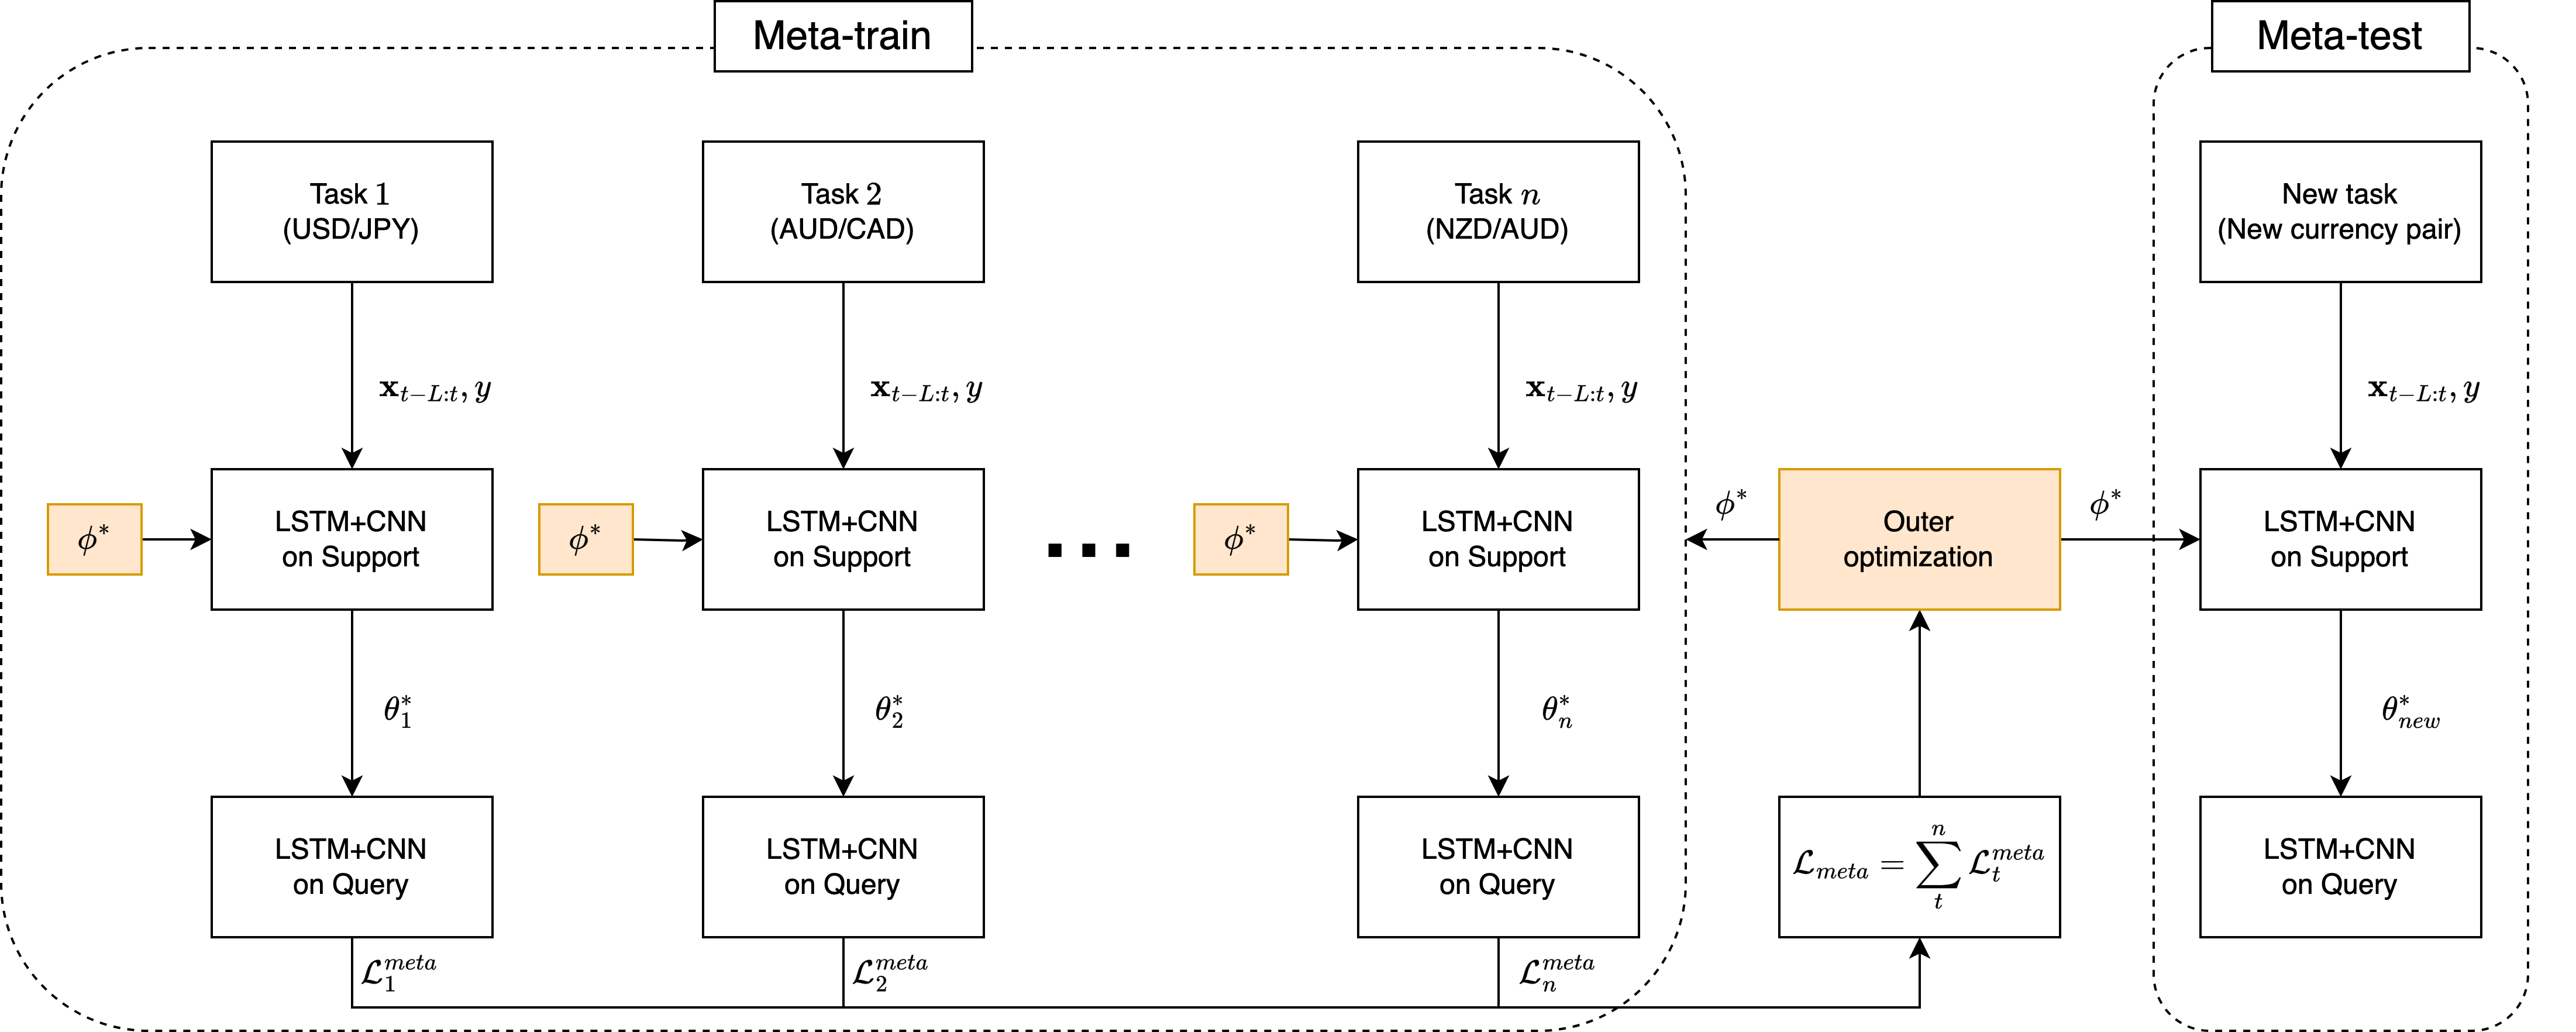
\includegraphics[width=\textwidth]{img/meta.png}
    \caption{The full-flow of meta-training and meta-testing on multi-fx data. Each currency pair is regarded as a task.}
    \label{fig:flow}
\end{figure*}

\subsection{Data preparation}

Phương pháp đề xuất sử dụng các thuật toán ML để huấn luyện mô hình. Do đó, dữ liệu cần được tổ chức lại để các thuật toán ML có thể hoạt động được. Trong trường hợp dữ liệu bao gồm nhiều datasets khác nhau thuộc cùng một lĩnh vực, mỗi dataset sẽ được coi là một task của \verb|MAML|. Trong trường hợp dữ liệu bao gồm một dataset duy nhất, cần chia nhỏ dataset này thành các tập con ứng với các task riêng biệt. Tóm lại, tập dữ liệu sau khi chuẩn bị bao gồm $n$ tasks: $\mathcal{D} = \left\{ \mathcal{D}_t \right\}_{t=1}^{n}$. Dữ liệu tại mỗi task được chia thành tập support và query: $\mathcal{D}_t = \left\{ \mathcal{D}_t^{support}, \mathcal{D}_t^{query} \right\}$.

\vspace{2mm}

Một sample dữ liệu bao gồm các cặp giá trị $(\mathbf{x}_{t-L:t}, y)$. Trong đó, $\mathbf{x}_{t-L:t}$ bao gồm $L$ giá trị lịch sử tính từ thời điểm $t$ trở về trước; $y\in \{0,1\}$ là nhãn dữ liệu, thể hiện xu hướng giảm, hoặc tăng của mẫu dữ liệu $x_{t+1}$ so với $x_{t}$. Tùy vào từng bài toán và cách cài đặt mà các phần tử trong $\mathbf{x}_{t-L:t}$ có thể là các vector hoặc các scalar number. Ví dụ, đối với dữ liệu chứng khoán, $\mathbf{x}_{t-L:t}$ có thể chứa các vector dữ liệu $\vec x_i = (\text{open, low, high, close})$ hoặc chỉ một giá trị close price duy nhất.

% nói từng cái, có thể sẽ vẽ hình cụ thể cho từng cái
% method phải chỉ ra được đoạn nào giải quyết thách thức nào (đã nêu ở intro)

% đến đoạn thực nghiệm thì sẽ mô tả sâu quá trình tìm kiếm tham số, quá trình chia dữ liệu, tải dữ liệu ở phụ lục
% nhận xét: nhấn mạnh vào việc giải quyết 3 thách thức nêu ở intro

\subsection{Feature extraction}

Lấy cảm hứng từ nghiên cứu \cite{vo2017multi}, chúng tôi đề xuất kết hợp các đặc trưng rút trích được từ mạng \verb|LSTM| và \verb|CNN|. Cụ thể, chúng tôi đưa từng phần tử trong vector $\mathbf{x}_{t-L:t}$ qua một lớp \verb|MLP| có đầu ra lớn hơn số chiều của $\vec x_i, i\in[t-L, t]$ để phân giải thành các đặc trưng nhỏ $\vec x'_i$. Các đặc trưng này sau đó được truyền qua mạng \verb|LSTM| và \verb|CNN| để lần lượt rút trích các phụ thuộc thời gian dài hạn ($\mathbf{h}_{LSTM}$) và các đặc trưng thời gian cục bộ ($\mathbf{h}_{CNN}$). Để có thể khai thác tối đa các ràng buộc thời gian dài hạn, chúng tôi sử dụng \verb|BidirectionalLSTM| để rút trích từ hai phía của của $\mathbf{x}_{t-L:t}$. Toàn bộ quy trình rút trích đặc trưng được tóm tắt như sau:

\begin{align}
    \mathbf{x'}_{t-L:t} &= \mathbf{FullyConnected}\left( \mathbf{x'}_{t-L:t} \right)\\
    \mathbf{h}_{LSTM} &= \mathbf{BidirectionalLSTM}\left( \mathbf{x'}_{t-L:t} \right)\\
    \mathbf{h}_{CNN} &= \mathbf{Convolution1D}\left( \mathbf{x'}_{t-L:t} \right)
    \label{eq:feature}
\end{align}

\vspace{2mm}

Mạng \verb|LSTM| duy trì giá trị cell-state nhằm lưu trữ có chọn lọc các phụ thuộc dài hạn. Điều này rất thích hợp trong việc giải quyết các bài toán time-series data. Mặt khác, giá trị tương lai thường phụ thuộc rất lớn vào các giá trị lịch sử gần nhất. Chúng tôi đề xuất sử dụng mạng \verb|CNN| để nhấn mạnh các đặc trưng cục bộ, từ đó hướng một phần sự chú ý của mô hình vào các thời điểm nhất định. Do đó, phương pháp đề xuất không chỉ nhớ được các đặc trưng long-term mà còn highlight được các đặc trưng short-term.

\vspace{2mm}

Tiếp đến, $\mathbf{h}_{LSTM}$ và $\mathbf{h}_{CNN}$ được nối với nhau (phương trình \ref{eq:concat}) sau đó chuyển đến phần phân lớp của mạng NN (phương trình \ref{eq:clf}).

\begin{align}
    \mathbf{h}_{t-L:t} &= \mathbf{Concatenate}\left( \mathbf{h}_{LSTM}, \mathbf{h}_{CNN} \right) \label{eq:concat} \\
    \hat y &= \mathbf{FullyConnected}\left( \mathbf{h}_{t-L:t} \right) \label{eq:clf}
\end{align}

\subsection{Effective synthesis\\of models' parameters}

Chúng tôi sử dụng \verb|MAML| để huấn luyện và tổng hợp trọng số của các mô hình tại các task. Như đã đề cập trong phần \ref{sec.relatedWork}, tối ưu tham số theo cách tiếp cận của ML chính là đi giải hai phương trình \ref{eq:inner_opt} và \ref{eq:outer_opt} bằng các phương pháp tối ưu trên dữ liệu support và query. Cụ thể, quá trình tối ưu bao gồm nhiều bước toàn cục (outer optimization), thực hiện trên tất cả các tasks tham gia huấn luyện. Mỗi bước toàn cục bao gồm nhiều bước cục bộ (inner optimization) thực hiện trên từng task riêng lẻ. Tại bước toàn cục $r$, quá trình tối ưu cục bộ lần thứ $e$ tại tập support của task $t$ diễn ra như sau:

\begin{align}
    \begin{cases}
        \theta_t^{(0)} &= \phi_{r-1} \\
        \theta_t^{(e)} &= \theta_t^{(e-1)} - \alpha \nabla_{\theta} \mathcal{L}^{task}_t\left( \theta_t^{(e-1)}, \mathcal{D}_t^{support} \right)
    \end{cases}
\end{align} Trong đó, $\phi_{r-1}$ là kết quả của quá trình tối ưu toàn cục lần thứ $r-1$, $\alpha$ là inner learning rate.

Tiếp đó, quá trình outer optimization tại bước toàn cục được thực hiện bằng cách tổng hợp độ lỗi trên tập query của các task và tối ưu trên đó (phương trình \ref{eq:outer_sol}).

\begin{align}
    \begin{cases}
        \phi_0 = \text{Random Initialization}\\
        \phi_r = \phi_{r-1} - \beta \nabla_{\phi} \sum_{t=1}^n{\mathcal{L}^{meta}_t \left( \theta_t^*(\phi), \mathcal{D}_t^{query} \right)}
    \end{cases}
    \label{eq:outer_sol}
\end{align} Trong đó, $\beta$ là outer learning rate. Giả sử thuật toán chạy $E$ steps trong inner optimization, lượng đạo hàm tại phương trình \ref{eq:outer_sol} được viết lại như sau (the notations of dataset are removed):

\begin{align*}
    &\beta \nabla_{\phi} \sum_{t=1}^n{\mathcal{L}^{meta}_t \left( \theta_t - \alpha \nabla_{\theta} \mathcal{L}^{task}_t\left( \theta_t \right) \right)}\\
    = &\beta \sum_{t=1}^n{ \frac{\partial \mathcal{L}^{meta}_t\left(\theta_t^{(E)}\right)}{\partial \theta_t^{(E)}} \frac{\partial \theta_t^{(E)}}{\partial \phi}}\\
    = &\beta \sum_{t=1}^n{ \nabla_{\theta} \mathcal{L}^{meta}_t\left(\theta_t^{(E)}\right) \prod_{j=0}^{E-1} {\left[\mathbb{I} - \alpha\nabla^2_{\theta}\mathcal{L}^{task}_{t}\left(\theta_t^{(j)}\right)\right]}} \numberthis
    \label{eq:outer_sol_}
\end{align*}

Sự xuất hiện của tích các đạo hàm bậc hai trong phương trình \ref{eq:outer_sol_} khiến quá trình đạo hàm trở nên phức tạp vì phải tốn rất nhiều chi phí để duy trì các ma trận Hessian. Do đó, số bước tính toán để tìm ra $\theta^*$ cần phải hạn chế. Trên thực tế, các phương pháp sử dụng ML \citep{fallah2020personalized, chen2018federated, nguyen2022meta,finn2017model, li2017meta} thường sẽ chọn $E\in [1,5]$.

%%%%%%%%%%%%%%%%%%%%%%%%%%%%%%%%%%%%%%%%%
\section{Numerical experiment}
\label{sec.experiment}
%%%%%%%%%%%%%%%%%%%%%%%%%%%%%%%%%%%e%%%%%%

\subsection{Dataset \& Metric}

FX nói riêng và các chỉ số tài chính nói chung là dạng dữ liệu điển hình cho aperiodic time-series data. Do đó, chúng tôi chọn loại dữ liệu này để kiểm thử mô hình. Cụ thể, chúng tôi cấu hình hai bộ dữ liệu sử dụng dữ liệu FX. Bộ dữ liệu \verb|USD/JPY| chỉ gồm dữ liệu của cặp tiền tệ USD/JPY, được chia thành 60 tập dữ liệu con theo trình tự thời gian với kích thước bằng nhau. Dữ liệu được sample theo giờ từ năm 2000 đến năm 2024, bao gồm các thuộc tính open, low, high, và close price. Bộ dữ liệu \verb|multi-fx| bao gồm 60 cặp tiền tệ giữa 18 quốc gia Australia, Canada, Switzerland, Denmark, EU, United Kingdom, Hong Kong, Iceland, Japan, Norway, New Zealand, Singapore, Sweden, Turkey, United States, Mexico, China, South Africa. Dữ liệu có thuộc tính tương tự như \verb|USD/JPY| và được sample theo ngày từ năm 2014 đến 2024. Số lượng mẫu dữ liệu của hai tập dữ liệu là tương đương nhau và xấp xỉ $156000$ mẫu.

\vspace{2mm}

Bộ dữ liệu \verb|multi-fx| được sử dụng để rút trích và tổng hợp thông tin về các yếu tố ngoại lai (i.e. thông tin thị trường, kinh tế, chính trị,...), vốn được cho là có ảnh hưởng đến kết quả của một chỉ số tài chính nhất định \citep{overreactioncontrarian,fama1970efficient,mech1993portfolio}. Bộ dữ liệu \verb|USD/JPY| được sử dụng để kiếm chứng giả thuyết của chúng tôi về việc dữ liệu tương lai ngầm phụ thuộc vào các thời điểm nhất định trong quá khứ và cần phải tổng hợp đặc trưng quá khứ một cách hiệu quả để làm rõ được các phụ thuộc này.

\vspace{2mm}

Nghiên cứu sử dụng macro accuracy, macro precision, macro recall, và macro F1 để đánh giá các mô hình. Theo đó, trong quá trình inference, mô hình sẽ chạy trên từng task để tính metrics của mỗi task. Sau đó tính trung bình cộng các metrics của các task để thu được kết quả cuối.

\subsection{Experiment}

Chúng tôi tiến hành so sánh phương pháp đề xuất với mô hình \verb|NHITS| thông qua các metrics nêu trên. Dữ liệu tổng quan được cấu trúc thành training sets, validation sets, và testing sets với tỷ lệ 6:2:2. Tập train dùng để huấn luyện mô hình, tập validation dùng để tìm kiếm siêu tham số và tập test để đánh giá mô hình. Đối với \verb|NHITS|, chúng tôi chia dữ liệu như bình thường theo tỷ lệ định sẵn ở trên. Đối với thuật toán đề xuất, vì quá trình meta-training và meta-testing đòi hỏi phải chia dữ liệu thành các task nhỏ, và cho phép mô hình adapt trên tập support của mỗi task, chúng tôi chia dữ liệu thành 60 tasks. Trong mỗi task, tập support chiếm 20\% với mục đích để mô hình học cách thích ứng với dữ liệu, tập query chiếm 80\% để kiểm tra khả năng tương thích của mô hình. Chúng tôi sử dụng 30 tasks để meta-train, 15 tasks để meta-validate, 15 tasks để meta-test. Với cách chia này, chúng tôi đảm bảo được tính công bằng khi mô hình ML được huấn luyện với lượng dữ liệu tương đương mô hình \verb|NHITS|.

%%%%%%%%%%%%%%%%%%%%%%%%%%%%%%%%%%%%%%%%%%%%%%%%
\section{Results and discussion}
\label{sec.results}
%%%%%%%%%%%%%%%%%%%%%%%%%%%%%%%%%%%%%%%%%%%%%%%%



\begin{table*}
    \centering
    \caption{meo meo}
    \begin{tblr}{
    cells = {c},
    cell{1}{2} = {c=4}{},
    cell{1}{6} = {c=4}{},
    vline{2-3} = {1}{},
    vline{2,6} = {2-4}{},
    hline{1,5} = {-}{0.08em},
    hline{2} = {2-9}{},
    hline{3} = {-}{},
    }
        & USD/JPY    &             &          &             & multi-fx     &              &             &               \\
        & $accuracy$ & $precision$ & $recall$ & $F_1-score$ & $accuracy$   & $precision$  & $recall$    & $F_1-score$   \\
    NHITS &            &             &          &             &              &              &             &               \\
    Ours  &            &             &          &             & $62.39±0.06$ & $71.11±9.34$ & $70.14±9.6$ & $69.21±11.07$ 
    \end{tblr}
    \label{tab:rs}
\end{table*}

% nói 1 chút về việc xài lstm+cnn/meta-learning sẽ giảm sự phụ thuộc của kết quả vào mạng NN/siêu tham số
% cụ thể, khi xài ML, tham số finetune rất dễ, cái nào cũng cao, chỉ cần chọn ra cái cao nhất
% giải thích tại sao cnn perform poorly: quá chú ý đến đặc trưng cục bộ mà quên mất các phụ thuộc dài hạn

%%%%%%%%%%%%%%%%%%%%%%%%%%%%%%%%%%%%%%%%%
\section{Conclusion \& Future direction}
\label{sec.conc}

% cite Meta-SGD, và 1 đống ML method vào đây để kiểu *ML có nhiều phương pháp, cần chạy thực nghiệm nhiều hơn
% cite iMAML, Reptile vào đây để làm future direction kiểu tối ưu lại ML vì chi phí hơi đắt

%%%%%%%%%%%%%%%%%%%%%%%%%%%%%%%%%%%%%%%%%

% Conclusion

%%%%%%%%%%%%%%%%%%%%%%%%%%%%%%%%%%%%%%%%%
\section{Acknowledgements}
%%%%%%%%%%%%%%%%%%%%%%%%%%%%%%%%%%%%%%%%%
% The work was carried out within the state assignment of Ministry of Science and Higher Education of the Russian Federation (No. AAAA-A18-118020190095-4, topic ``Quantum''). G.I.P is grateful for financial supports from JST SPRING, Grant Number JPMJSP2102. K. H. is grateful for financial support from MEXT-KAKENHI (JP19K05029, JP21K03400, JP21H01998, and JP22H02170). R.M. is grateful for financial supports from MEXT-KAKENHI (22H05146, 21K03400 and 19H04692).

%%%%%%%%%%%%%%%%%%%%%%%%%%%%%%%%%%%%%%%%%
\section{Author contributions}
%%%%%%%%%%%%%%%%%%%%%%%%%%%%%%%%%%%%%%%%%
% All authors contributed to conceiving the idea. T.I., A.V.U, and G.I.P performed the calculations. T.I. made the all figures. R.M and S.V.S supervised the work. All authors contributed to the discussion and writing of the paper.

%%%%%%%%%%%%%%%%%%%%%%%%%%%%%%%%%%%%%%%%%
\section{Data availability statement}
%%%%%%%%%%%%%%%%%%%%%%%%%%%%%%%%%%%%%%%%%
% The datasets used and/or analyzed during the current study available from the corresponding authors on reasonable request.

%%%%%%%%%%%%%%%%%%%%%%%%%%%%%%%%%%%%%%%%%
\bibliographystyle{elsarticle-harv} 
\bibliography{references}
\end{document}
%%%%%%%%%%%%%%%%%%%%%%%%%%%%%%%%%%%%%%%%%



%%%%%%%%%%%%%%%%%%%%%%%%%%%%%%%%%%%%%%%%%%
%\section{Appendix}
%%%%%%%%%%%%%%%%%%%%%%%%%%%%%%%%%%%%%%%%%%
%We used the VASP code\cite{VASP} for the calculations explained in this appendix.
%We relaxed the four structures of Figure \ref{fig.str}
%for every LiV$X_2$ ($X$ = O, S, and Se) with each of PBE\cite{PBE},
%optPBE-vdW-DF\cite{2009JK_AM,vdW-DFa,vdW-DFb}, and HSE06\cite{HSE06} functionals.
%We evaluated the relative energies of structures relaxed by every functional by PBE-DFT.
%%as shown in Figure \ref{fig.geomErr}.
%We found that the differences of the relative energies
%among the structures relaxed by different functionals are at most 0.018 eV/f.u.
%%the differences of the time-series in Figure \ref{fig.geomErr} are within 0.018 eV/f.u.

%%----------------------------------------
%\begin{figure}[htbp]
%  \centering
%  \includegraphics[width=\hsize]{geomErr.eps}
%  \caption{\ghost{fig.geomErr}\label{fig.geomErr}
%    FNDMC and DFT results of relative energies of the four candidate structures
%    of LiV$X_2$ (X = O, S, and Se).
%    The candidate structures are shown in Figure \ref{fig.str}.
%    TR-I and TR-II (left from the vertical line) are trimmerized
%    and NTR-I and NTR-II (right from the vertical line) are
%    non-trimmerized structures, respectively.
%    FNDMC results are same as Figure \ref{fig.dmconly}.
%    The lowest energy among the four structures is set to be zero
%    and the others are given as relative values from the lowest energy.
%  }
%\end{figure}
%%----------------------------------------
